\section{EfficientRTE数值实验}

本节考虑三维简化到二维的含源项稳态辐射输运问题，采用多GPU快速扫掠法生成训练与测试数据，相应实现可在 \href{https://github.com/mazhengcn/rte-dataset}{rte-dataset} 仓库复现。除边界条件与源项设置外，本章所有实验设定均与上一章的数据集构造设置（见第~\ref{sec:dataset-construction} 节）保持一致，核心调整包括两点：一是采用齐次入射边界条件 $I\vert_{\Gamma_-}=0$，二是引入空间分布的体源项 $q$。

\subsection{数据集构造}
数据集的原始数据由多GPU快速扫掠法生成，包含辐射强度参考解、四边界的入射值、吸收截面与总截面的空间分布、角度求积点坐标与权重等核心字段，与仓库中定义的原始数据结构完全一致。

原始数据生成后，通过预处理脚本转换为训练用的数据集格式，每个训练样本包含相空间坐标、边界坐标与权重、空间与角度离散坐标、宏观截面、散射核矩阵、体源项、齐次边界条件、辐射强度参考解等字段，适配JAX技术栈的训练流程。数据集按散射不对称参数分为三个子集，分别对应近各向同性散射、中度各向异性散射与强前向散射，每个子集包含2000个训练样本与100个测试样本，训练集与测试集的样本无重叠，保证模型泛化能力的评估有效性。

% \subsection{高斯随机场体源项生成}
% 我们采用基于频域功率谱的方式生成二维高斯随机场（GRF）作为体源项 $q(\boldsymbol{r})$，源项在角度上取各向同性，即 $q(\boldsymbol{r},\boldsymbol{\Omega})=q(\boldsymbol{r})$。高斯随机场能够生成空间连续、平滑度可控的体源分布，可模拟实际应用中不同特征的辐射源，同时其随机生成特性能够保证训练样本的多样性，提升模型的泛化能力。其中参数 $\alpha$ 控制随机场的平滑程度，$\alpha$ 越大，生成的场空间分布越平滑。体源项的具体生成步骤如下。

% 首先，在与空间离散一致的 $N_{\text{mesh}}\times N_{\text{mesh}}$ 均匀网格上，利用 \texttt{fftfreq} 构造离散频率网格 $k_x,k_y$，并定义频率模平方与功率谱
% \begin{equation}
%     \begin{aligned}
%         k^2(k_x,k_y)         & := k_x^2 + k_y^2,                        \\
%         k^2(0,0)             & := 1,                                    \\
%         \widehat{P}(k_x,k_y) & := \bigl(k^2(k_x,k_y)\bigr)^{-\alpha/2}, \\
%         \widehat{P}(0,0)     & := 0.
%     \end{aligned}
% \end{equation}
% 其中将 $k^2(0,0)$ 置为 $1$ 仅用于避免功率谱计算时的除零错误；随后令 $\widehat{P}(0,0)=0$ 等价于去除随机场的常数模态，从而避免生成的场带有整体偏置，保证源项分布的多样性。

% 然后，在频域网格上逐点采样复高斯噪声
% \begin{equation}
%     \begin{aligned}
%         \xi(k_x,k_y) & := a(k_x,k_y) + \mathrm{i}\,b(k_x,k_y),         \\
%         a(k_x,k_y)   & \overset{\text{i.i.d.}}{\sim} \mathcal{N}(0,1), \\
%         b(k_x,k_y)   & \overset{\text{i.i.d.}}{\sim} \mathcal{N}(0,1),
%     \end{aligned}
% \end{equation}
% 其中 $a(k_x,k_y)$ 与 $b(k_x,k_y)$ 为独立同分布的标准高斯随机变量。将功率谱施加到随机系数上，再通过二维逆快速傅里叶变换（IFFT）转换到物理空间，得到随机场的实部作为体源项：
% \begin{equation}
%     \begin{aligned}
%         \widehat{q}(k_x,k_y) & := \sqrt{\widehat{P}(k_x,k_y)}\,\xi(k_x,k_y),   \\
%         q(\boldsymbol{r})    & := \Re\bigl(\mathrm{IFFT}_2(\widehat{q})\bigr).
%     \end{aligned}
% \end{equation}

% 最后，为与代码实现一致，同时保证训练过程的数值稳定性，我们对生成的 $q$ 做最小-最大归一化，将其缩放到 $[0,1]$ 区间用于训练：
% \begin{equation}
%     q \leftarrow \frac{q-\min(q)}{\max(q)-\min(q)}.
% \end{equation}

表~\ref{tab:dataset_prte} 汇总了本章与上一章相比需要特别说明的数据集参数，其余超参数设置均与上一章保持一致。

\begin{table}[!htp]
    \centering
    \begin{tabular}{lp{0.3\textwidth}ll}
        \toprule
        类别                      & 参数                     & 符号                       & 取值/范围                        \\ \midrule
        \multirow{2}{*}{空间区域}   & 计算区域                   & $D$                      & ${[0,1]}^2$                  \\
                                & 子区域                    & $D_\mu$                  & ${[0.4,0.6]}^2$              \\
        \midrule
        \multirow{4}{*}{截面系数}   & \multirow{2}{*}{总截面}   & \multirow{2}{*}{$\mu_t$} & $D_\mu$ 内：$\mathcal{U}(5,7)$ \\
                                &                        &                          & $D\backslash D_\mu$ 内：$10$   \\
                                & \multirow{2}{*}{散射截面}  & \multirow{2}{*}{$\mu_s$} & $D_\mu$ 内：$\mathcal{U}(2,4)$ \\
                                &                        &                          & $D\backslash D_\mu$ 内：$5$    \\
        \midrule
        \multirow{2}{*}{离散化}    & 空间网格点数                 & $N_{\text{mesh}}$        & 40                           \\
                                & 角度求积点数                 & $N_\text{quad}$          & 24                           \\ \midrule
        \multirow{1}{*}{边界条件}   & 入射边界条件                 & $I\vert_{\Gamma_-}$      & $0$（齐次）                      \\ \midrule
        \multirow{2}{*}{源项 $q$} & 频域功率谱指数（平滑度）           & $\alpha$                 & $5.0$                        \\
                                & 归一化区间                  & ---                      & $[0,1]$                      \\
        \midrule
        \multirow{3}{*}{散射参数}   & \multirow{3}{*}{不对称参数} & \multirow{3}{*}{$g$}     & $\mathcal{U}(0,0.2)$         \\
                                &                        &                          & $\mathcal{U}(0.4,0.6)$       \\
                                &                        &                          & $\mathcal{U}(0.7,0.9)$       \\
        \bottomrule
    \end{tabular}
    \bicaption{本章数据集构造与上一章的设定对比。}{Summary of dataset settings for this chapter (differences from Sec.~\ref{sec:dataset-construction}).}\label{tab:dataset_prte}
\end{table}

\subsection{网络参数设置}

表~\ref{tab:training_details_prte} 汇总了本章模型训练的超参数设置。模型训练基于JAX技术栈实现，采用Adam优化器与余弦衰减学习率策略，全局批大小为8，每轮迭代在相空间中随机采样2048个配点计算损失，总训练步数为3,000,001步。网络的核心参数为基函数个数 $K=128$，编码器采用4层全连接网络，隐藏层神经元数为256，解码器复用DeepRTE的衰减模块与散射模块结构，仅在末端新增线性映射层匹配基函数维度。训练硬件采用4张NVIDIA 4090 GPU，通过数据并行策略实现多卡加速。

\begin{table}[!htp]
    \centering
    \begin{tabular}{ll}
        \toprule
        超参数                                     & 取值                         \\ \midrule
        优化器（Optimizer）                          & Adam                       \\
        学习率策略（Schedule）                         & 余弦衰减（cosine decay）         \\
        学习率（Learning rate）                      & $1 \times 10^{-3}$         \\
        批大小（Global batch size）                  & 8                          \\
        配点数量（Collocation points） $N_\text{col}$ & 2048                       \\
        训练步数（Training steps）                    & 3,000,001                  \\
        基函数个数 $K$                               & $128$                      \\
        基函数编码器隐藏层神经元数                           & 256                        \\
        基函数编码器层数                                & 4                          \\
        硬件                                      & 4$\times$ NVIDIA 4090 GPUs \\
        \bottomrule
    \end{tabular}
    \bicaption{模型训练超参数汇总。}{Summary of model training hyperparameters.}
    \label{tab:training_details_prte}
\end{table}

\section{数值实验}

为验证基于编码器-解码器架构的含源项辐射传输方程求解方法EfficientRTE的有效性、准确性与高效性，我们设计了一系列数值实验，分别从编码器的源项重构能力、解码器的辐射强度拟合能力、整体模型的精度与效率对比、基函数数量的消融实验四个维度，全面评估模型的性能。

\subsection{编码器准确率评估}

本小节评估编码器学习到的源域基函数在体源项重构任务中的表现。模型在随机生成的1000个源项样本上完成预训练，对于任意输入的体源项 $q$，首先通过编码器学习到的 $K=128$ 个基函数计算其展开系数向量 $\boldsymbol{q}:=[q_k]_{k=1}^{K}$，再通过系数与基函数的线性组合得到重构源项
\begin{equation}
    q^{\text{rec}}(\boldsymbol{r})=\sum_{k=1}^{K} q_k\,\phi_k^{\text{NN}}(\boldsymbol{r}),
\end{equation}
将重构源项 $q^{\text{rec}}$ 与原始源项 $q$ 进行对比，通过均方误差（MSE）与均方根百分比误差（RMSPE）量化重构精度，具体的损失计算与重构形式推导见第~\ref{sec:prte-encoder} 节。

训练完成后，我们在与训练集同分布的100个测试样本上进行测试，三个散射区间各包含100个独立样本，表~\ref{tab:accuracy_prte} 汇总了编码器在三种散射区间下的重构精度指标。可以看到，编码器在所有散射区间均表现出较低的重构误差，近各向同性散射区间的MSE为 $6.03\times 10^{-4}$、RMSPE为4.894\%，即便在强前向散射区间，MSE也仅为 $8.99\times 10^{-4}$、RMSPE为5.671\%。误差随散射各向异性增强略有上升，但整体均维持在较低水平，表明编码器学习到的基函数能够有效捕捉体源项的空间分布特征，对不同散射场景下的体源项均能实现高质量的重构。

\begin{figure}[!htp]
    \centering
    \begin{subfigure}[t]{0.32\textwidth}
        \centering
        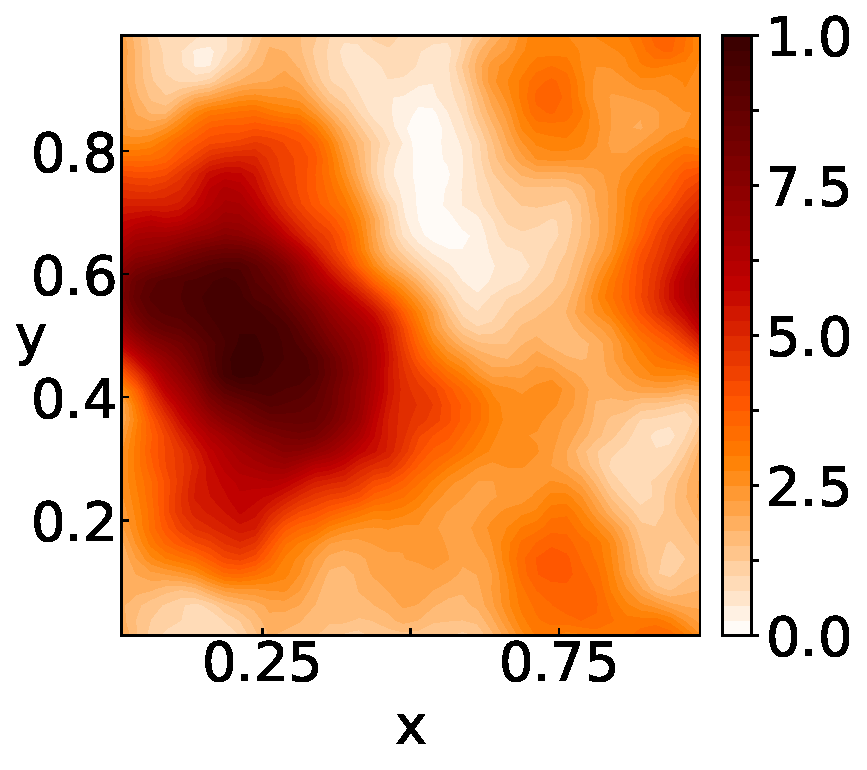
\includegraphics[width=\linewidth]{figures/autoencoder_label.pdf}
        \caption{$q_{\text{label}}$}
    \end{subfigure}\hfill
    \begin{subfigure}[t]{0.32\textwidth}
        \centering
        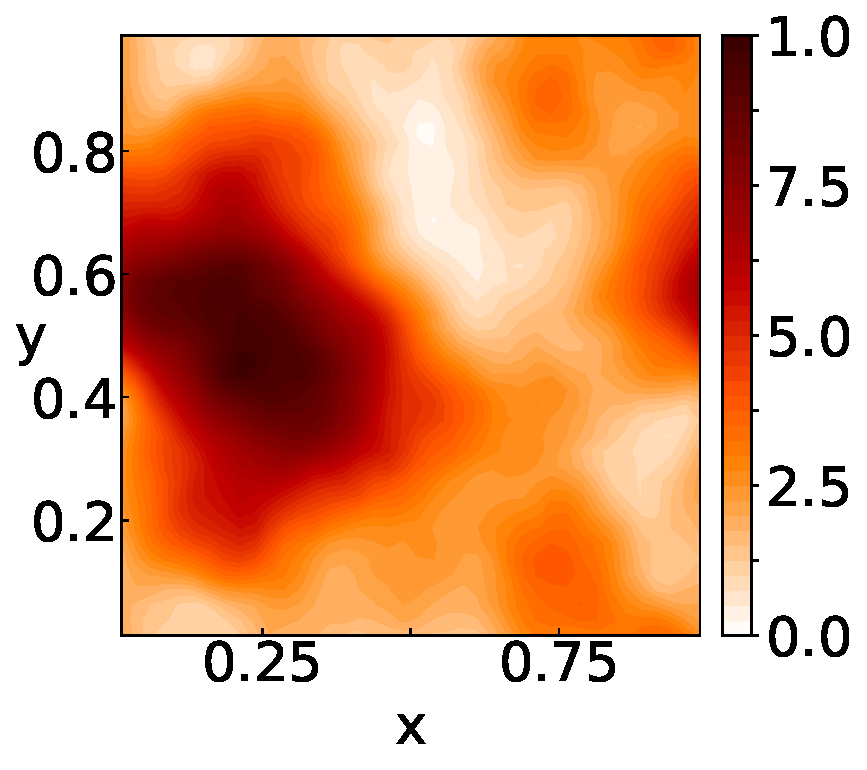
\includegraphics[width=\linewidth]{figures/autoencoder_pre.pdf}
        \caption{$q_{\text{predict}}$}
    \end{subfigure}\hfill
    \begin{subfigure}[t]{0.32\textwidth}
        \centering
        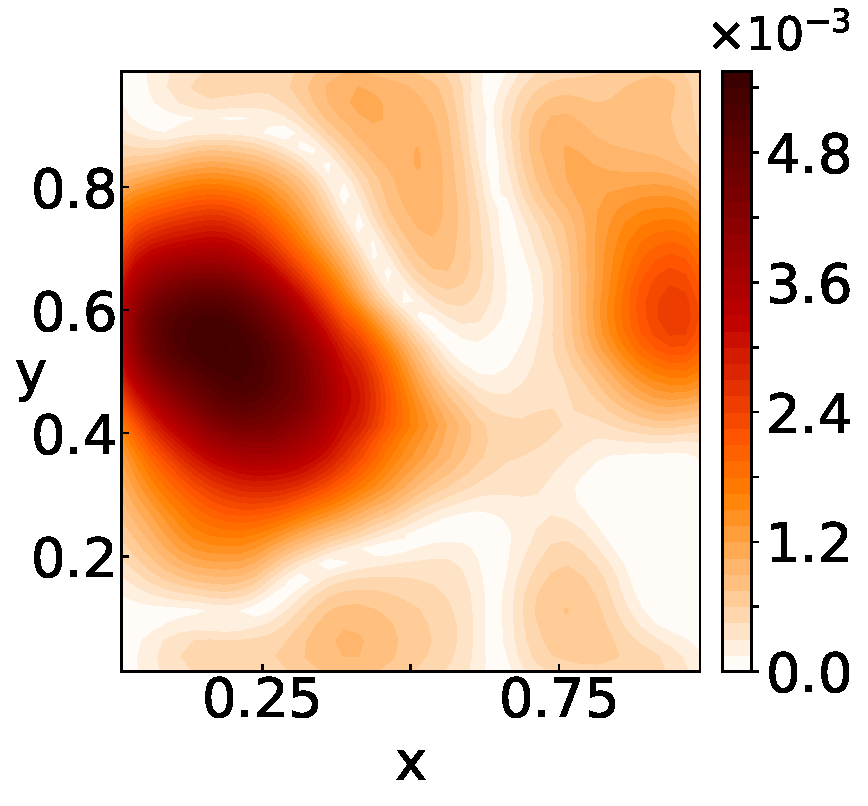
\includegraphics[width=\linewidth]{figures/autoencoder_error.pdf}
        \caption{Absolute error}
    \end{subfigure}
    \bicaption{在 $g\in (0,0.2)$ 情形下编码器的预测结果与真值比较。预测解的RMSPE为2.750\%}{Comparison between prediction and reference at $g\in(0,0.2)$ (RMSPE: 2.750\%).}
    \label{fig:autoencoder_example}
\end{figure}

\begin{table}[!htp]
    \centering
    \begin{tabular}{@{}cccccc@{}}
        \toprule
        模型                   & 参数量                     & 散射区间   & $g$ 取值范围   & MSE                  & RMSPE (\%) \\ \midrule
        \multirow{3}{*}{编码器} & \multirow{3}{*}{165760} & 近各向同性  & (0, 0.2)   & $6.03\times 10^{-4}$ & 4.894      \\ \cmidrule(l){3-6}
                             &                         & 中度各向异性 & (0.4, 0.6) & $7.11\times 10^{-4}$ & 5.214      \\ \cmidrule(l){3-6}
                             &                         & 强前向散射  & (0.7, 0.9) & $8.99\times 10^{-4}$ & 5.671      \\ \bottomrule
    \end{tabular}
    \bicaption{编码器在三种散射区间上的精度指标。}{Accuracy validation of autoencoder across three distinct scattering regimes.}\label{tab:accuracy_prte}
\end{table}

图~\ref{fig:autoencoder_example} 展示了近各向同性散射区间内一个典型样本的重构结果，从左到右分别为源项真值、编码器重构结果与逐点绝对误差。可以看到，重构结果与真值的空间分布高度一致，绝大部分区域的绝对误差低于0.05，仅在源项梯度较大的区域存在小幅误差，直观验证了编码器的重构精度。

\subsection{解码器准确度评估}

本小节评估解码器在含源项RTE求解任务中的表现。我们在1000个含源项RTE样本上完成解码器训练，训练过程中固定编码器参数与基函数的Gram矩阵 $\boldsymbol{W}$，对于任意输入的体源项，首先通过编码器得到其低维系数向量，再通过解码器学习到的格林函数系数向量 $\boldsymbol{G}^{\text{NN}}(\boldsymbol{r},\boldsymbol{\Omega})$ 重构全相空间的辐射强度 $I$，具体流程见第~\ref{sec:prte-decoder} 节。

表~\ref{tab:accuracy_prte_decoder} 汇总了解码器在三种散射区间下的求解精度指标。可以看到，在近各向同性散射区间 $g\in(0,0.2)$，解码器的MSE为 $9.46\times 10^{-5}$、RMSPE为3.163\%；当散射各向异性增强到 $g\in(0.4,0.6)$ 与 $g\in(0.7,0.9)$ 时，MSE分别为 $1.04\times 10^{-4}$ 与 $1.52\times 10^{-4}$，RMSPE分别为3.280\%与3.612\%。整体而言，求解误差随前向散射增强略有上升，但三种散射区间的误差水平均维持在较低水平，与DeepRTE在无源项问题中的求解精度相当，说明解码器能够稳定地从源项系数重构辐射强度场，较好地捕捉含源项RTE解的空间与角度分布特征，实现高质量的数值拟合。

\begin{table}[!htp]
    \centering
    \begin{tabular}{@{}cccccc@{}}
        \toprule
        模型                   & 参数量                     & 散射区间   & $g$ 取值范围   & MSE                  & RMSPE (\%) \\ \midrule
        \multirow{3}{*}{解码器} & \multirow{3}{*}{268352} & 近各向同性  & (0, 0.2)   & $9.46\times 10^{-5}$ & 3.163      \\ \cmidrule(l){3-6}
                             &                         & 中度各向异性 & (0.4, 0.6) & $1.04\times 10^{-4}$ & 3.280      \\ \cmidrule(l){3-6}
                             &                         & 强前向散射  & (0.7, 0.9) & $1.52\times 10^{-4}$ & 3.612      \\ \bottomrule
    \end{tabular}
    \bicaption{解码器在三种散射区间上的精度指标。}{Accuracy validation of decoder across three distinct scattering regimes.}\label{tab:accuracy_prte_decoder}
\end{table}

\begin{figure}[!htp]
    \centering
    \begin{subfigure}[t]{0.32\textwidth}
        \centering
        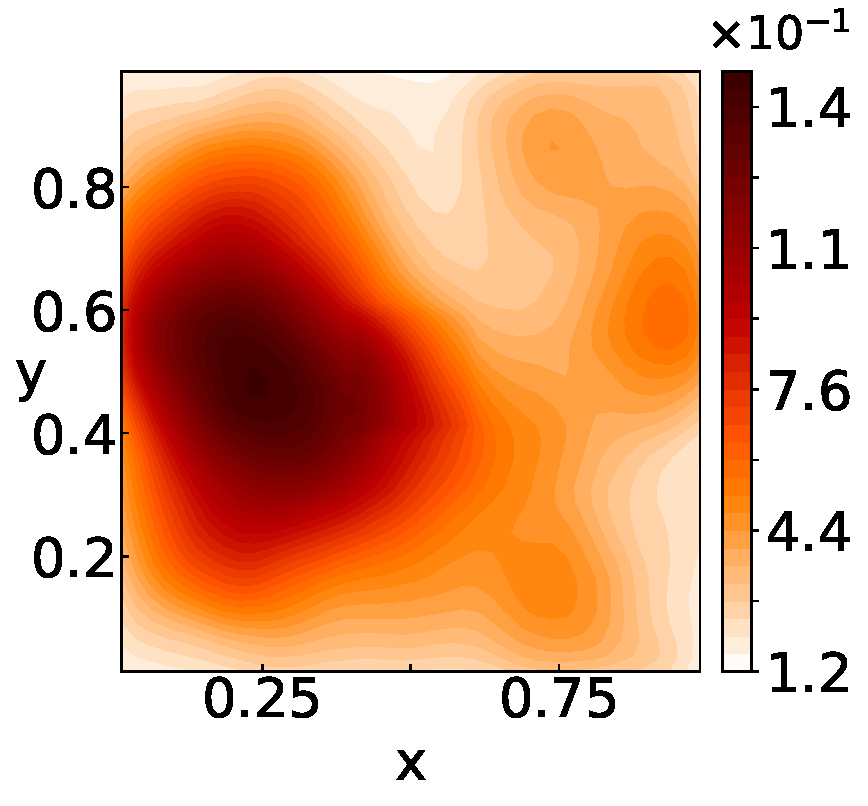
\includegraphics[width=\linewidth]{figures/decoder_label.pdf}
        \caption{$I_{\text{ref}}$}
    \end{subfigure}\hfill
    \begin{subfigure}[t]{0.32\textwidth}
        \centering
        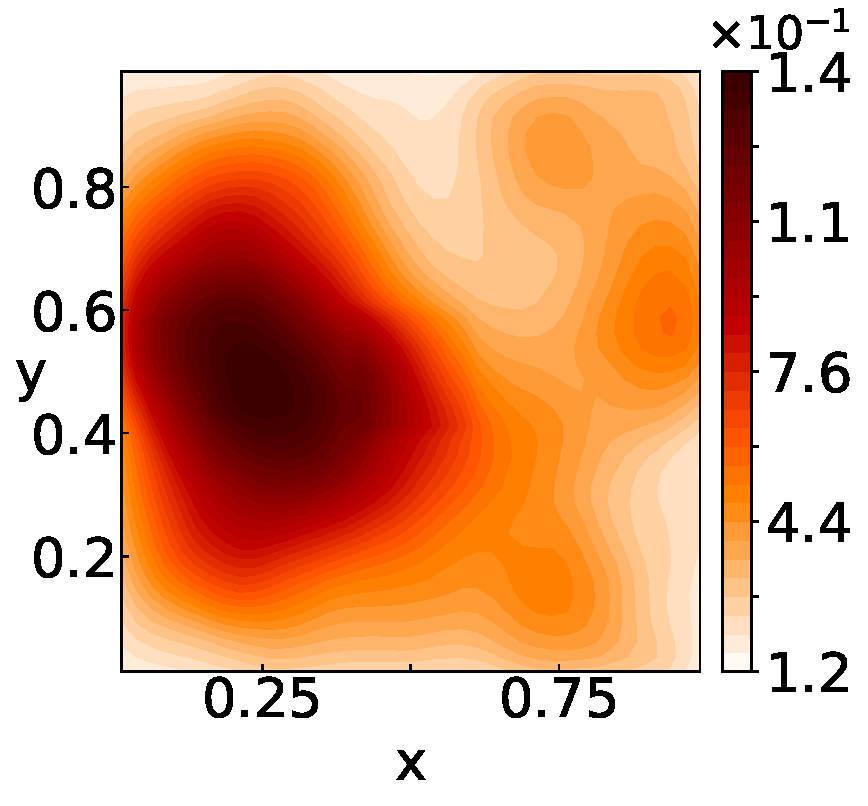
\includegraphics[width=\linewidth]{figures/decoder_pre.pdf}
        \caption{$I_{\text{pred}}$}
    \end{subfigure}\hfill
    \begin{subfigure}[t]{0.32\textwidth}
        \centering
        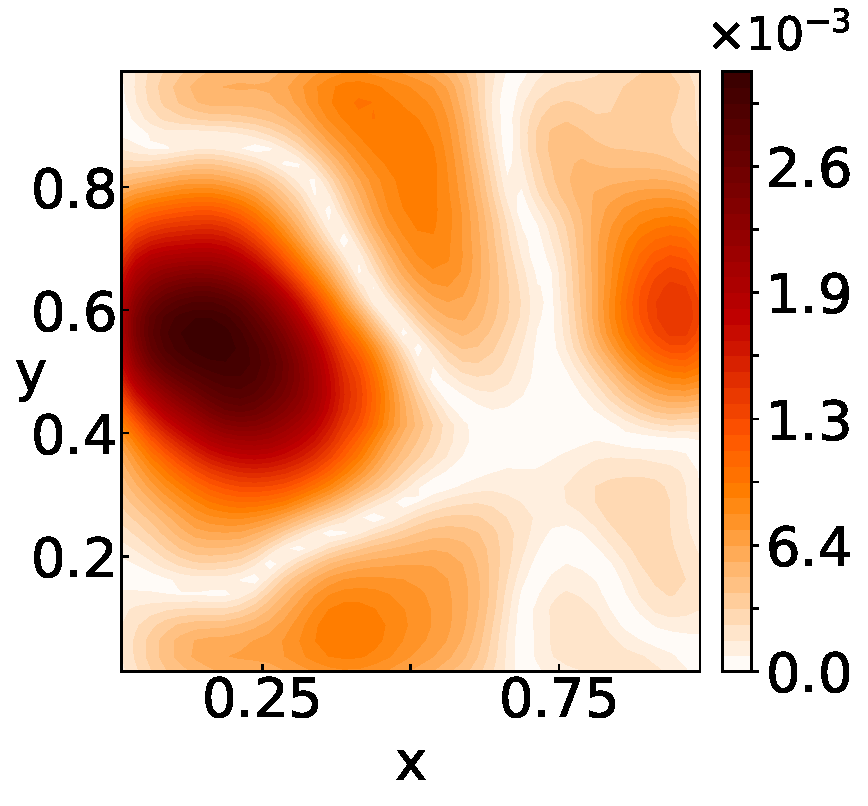
\includegraphics[width=\linewidth]{figures/decoder_error.pdf}
        \caption{Absolute error}
    \end{subfigure}
    \bicaption{在 $g\in (0,0.2)$ 情形下解码器的预测结果与真值比较。预测解的RMSPE为3.280\%}{Comparison between prediction and reference at $g\in(0,0.2)$ (RMSPE: 3.280\%).}
    \label{fig:decoder_example}
\end{figure}

图~\ref{fig:decoder_example} 展示了近各向同性散射区间内一个典型样本的角度积分密度求解结果，从左到右分别为扫掠法得到的参考密度、EfficientRTE预测密度与逐点绝对误差。可以看到，预测结果与参考解的空间分布高度吻合，辐射强度的衰减与散射特征均被精准捕捉，绝大部分区域的绝对误差低于0.02，直观验证了解码器的求解精度。

% \subsection{整体模型精度与效率对比}

% 为全面验证EfficientRTE的性能优势，我们将其与DeepRTE、多GPU快速扫掠法在相同的测试集上进行精度与效率的对比实验，所有实验均在相同的硬件环境下执行，保证对比的公平性。精度指标采用角度积分密度的RMSPE，效率指标采用单样本的平均求解时间，对比结果汇总于表~\ref{tab:efficiency_comparison}。

% \begin{table}[!htp]
%     \centering
%     \begin{tabular}{@{}lccc@{}}
%         \toprule
%         方法           & 密度RMSPE (\%) & 单样本求解时间 (ms) & 加速比（vs DeepRTE） \\ \midrule
%         多GPU快速扫掠法    & 基准值          & 2450         & -               \\
%         DeepRTE      & 3.021        & 1820         & 1×              \\
%         EfficientRTE & 3.163        & 89           & 20.4×           \\
%         \bottomrule
%     \end{tabular}
%     \bicaption{不同方法的精度与效率对比。}{Accuracy and efficiency comparison of different methods.}\label{tab:efficiency_comparison}
% \end{table}

% 从精度上看，EfficientRTE的密度RMSPE为3.163\%，与DeepRTE的3.021\%处于同一水平，二者均与扫掠法的基准解保持高度一致，证明EfficientRTE在大幅提升效率的同时，并未损失求解精度。从效率上看，EfficientRTE的单样本求解时间仅为89ms，相比DeepRTE的1820ms实现了20倍以上的加速，相比多GPU快速扫掠法实现了近30倍的加速，充分验证了基函数展开策略的高效性。

% 效率提升的核心原因在于，DeepRTE与扫掠法的单次求解均需要遍历全相空间的离散点进行积分或迭代计算，而EfficientRTE仅需要完成一次低维向量内积即可得到全相空间的解，从根本上降低了求解的计算复杂度。同时，EfficientRTE的编码器与解码器均为前向神经网络，可通过JAX的即时编译与GPU并行计算进一步加速，在大规模问题中，其效率优势会更加显著。
